\documentclass{standalone}
\usepackage{tikz-network}
\begin{document}
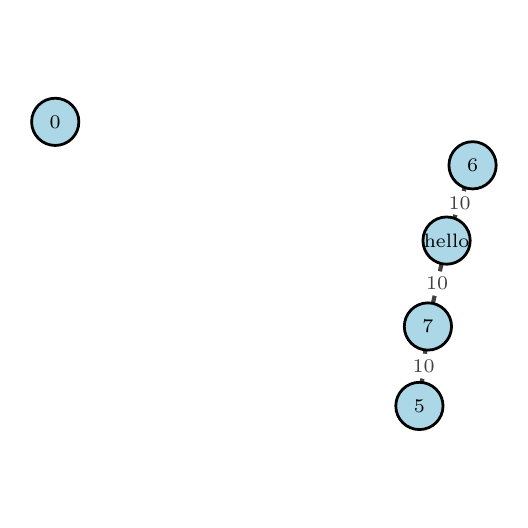
\begin{tikzpicture}
\clip (0,0) rectangle (6,6);
\Vertex[x=5.320,y=3.296,label=hello]{hello}
\Vertex[x=0.350,y=4.804,label=0]{0}
\Vertex[x=4.975,y=1.196,label=5]{5}
\Vertex[x=5.650,y=4.252,label=6]{6}
\Vertex[x=5.083,y=2.205,label=7]{7}
\Edge[,bend=0,label=10](hello)(6)
\Edge[,bend=0,label=10](hello)(7)
\Edge[,bend=0,label=10](5)(7)
\end{tikzpicture}
\end{document}